\chapter*{Annexe du chapitre \ref{chap:Comparaison}: Sélection des positions }
\label{chap:annexeproteus}

Cette annexe présente les principales structures de données utilisées dans le programme proteus. Un premier ensemble de structures regroupe les données physiques fournies en entrée à proteus, voir la figure \ref{fig:structPhy}. Le fichier backbone contient d'une part la description de tous les rotamères possibles de chaque position du système étudié. Et d'autre part les énergies propres de chacun de ces rotamères. La structure \verb!residues! contient la totalité de ces rotamères répartie en \verb!residue!. Ils sont regroupés dans un tableau \verb!rotamers!  pour chaque type qui est regroupé à leur tour dans un tableau \verb!types!. La matrice \verb!ener! regroupe les énergies de paires dans un tableau à deux dimensions représentant les couples de positions $(i,j)$. Chaque élément de ce tableau contenant l'ensemble des couples de rotamères de $(i,j)$  sous forme de tableau à deux dimensions également.

   \begin{figure}[!htbp]
     \centering
     \begin{tabular}{c}
       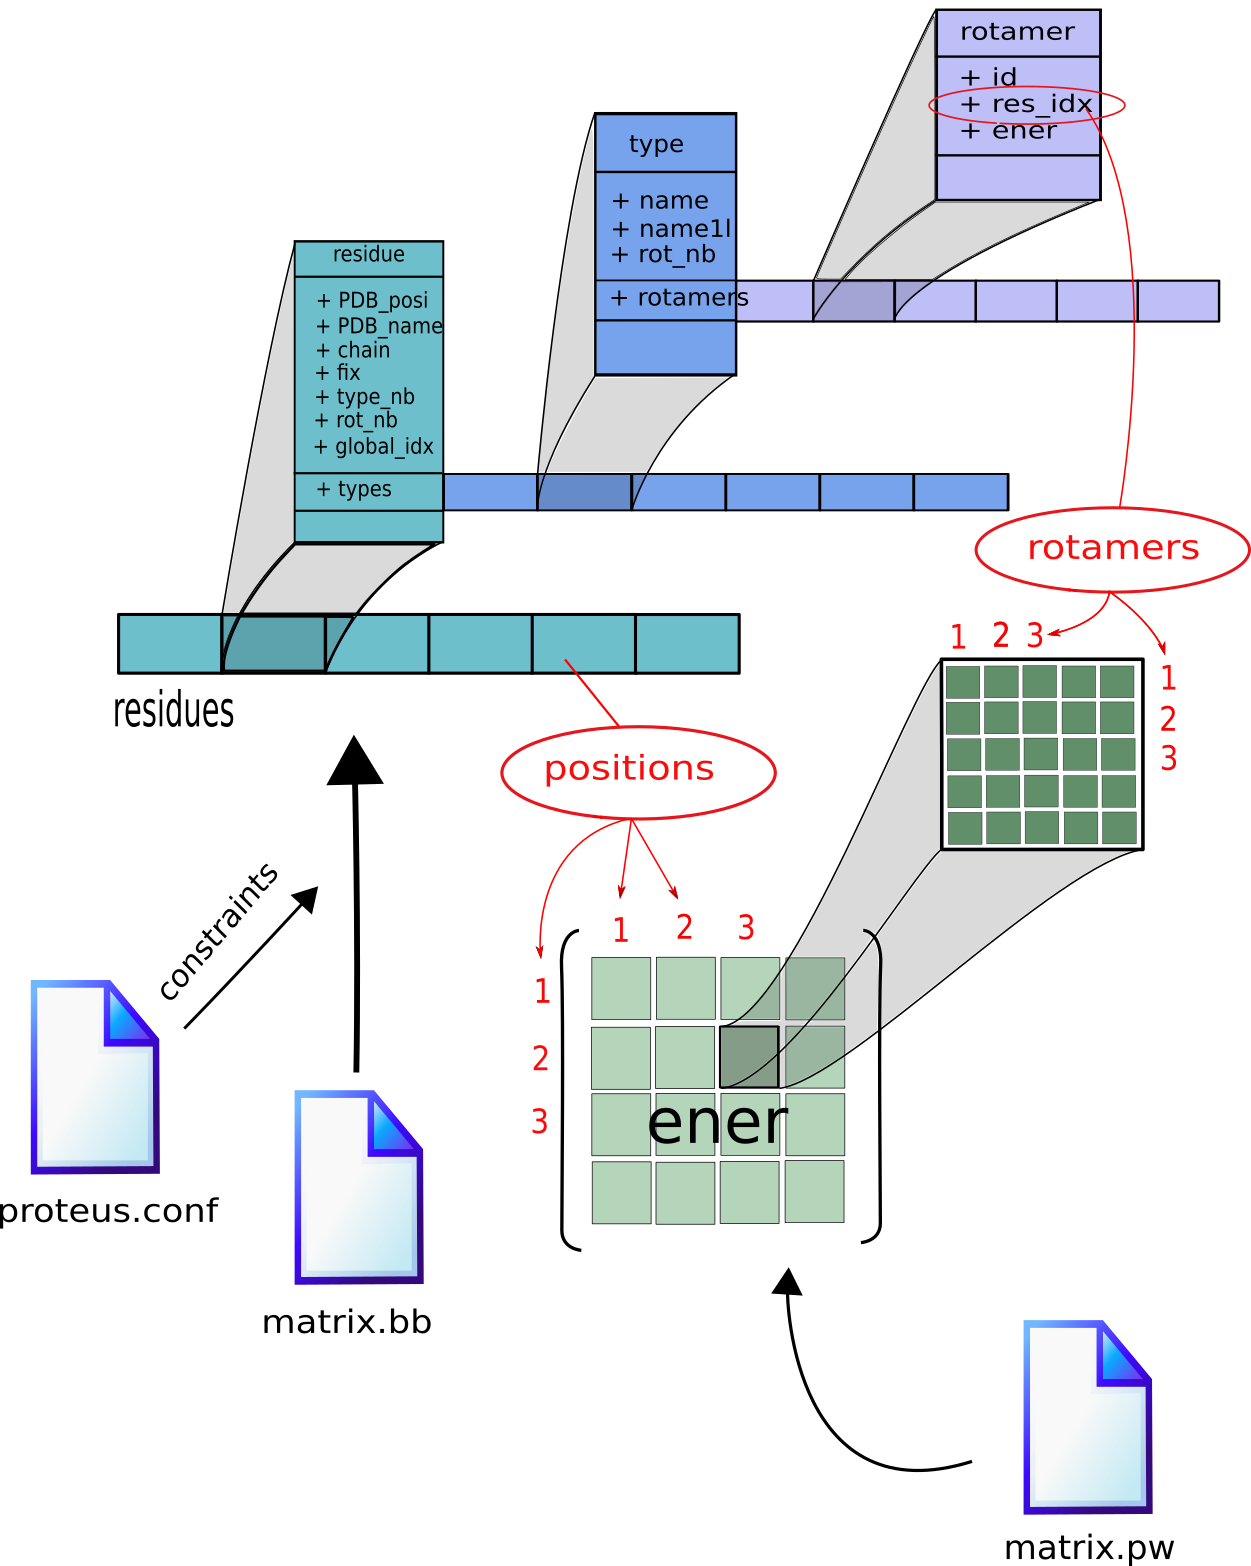
\includegraphics[width=12cm]{figure/structures_physique.png} 
     \end{tabular}
     
     \caption{Les principales structures \og physiques\fg dans proteus}
\label{fig:structPhy}
   \end{figure}

 Le deuxième ensemble de structures est constitué des structures \og logiques \fg. Ce sont elles qui gèrent la duplicité de parties du système comme expliqué dans \ref{sub:group}. La structure \verb!posi_instance! contient un ensemble d'index de tableaux \verb!rotamers! permettant la définition d'un espace d'état qui lui est propre. La structure \verb!group! contient à son tour une liste de \verb!posi_instance!. Cela est détaillé à la figure  \ref{fig:structLog}.   

 
   \begin{figure}[!htbp]
     \centering
     \begin{tabular}{c}
       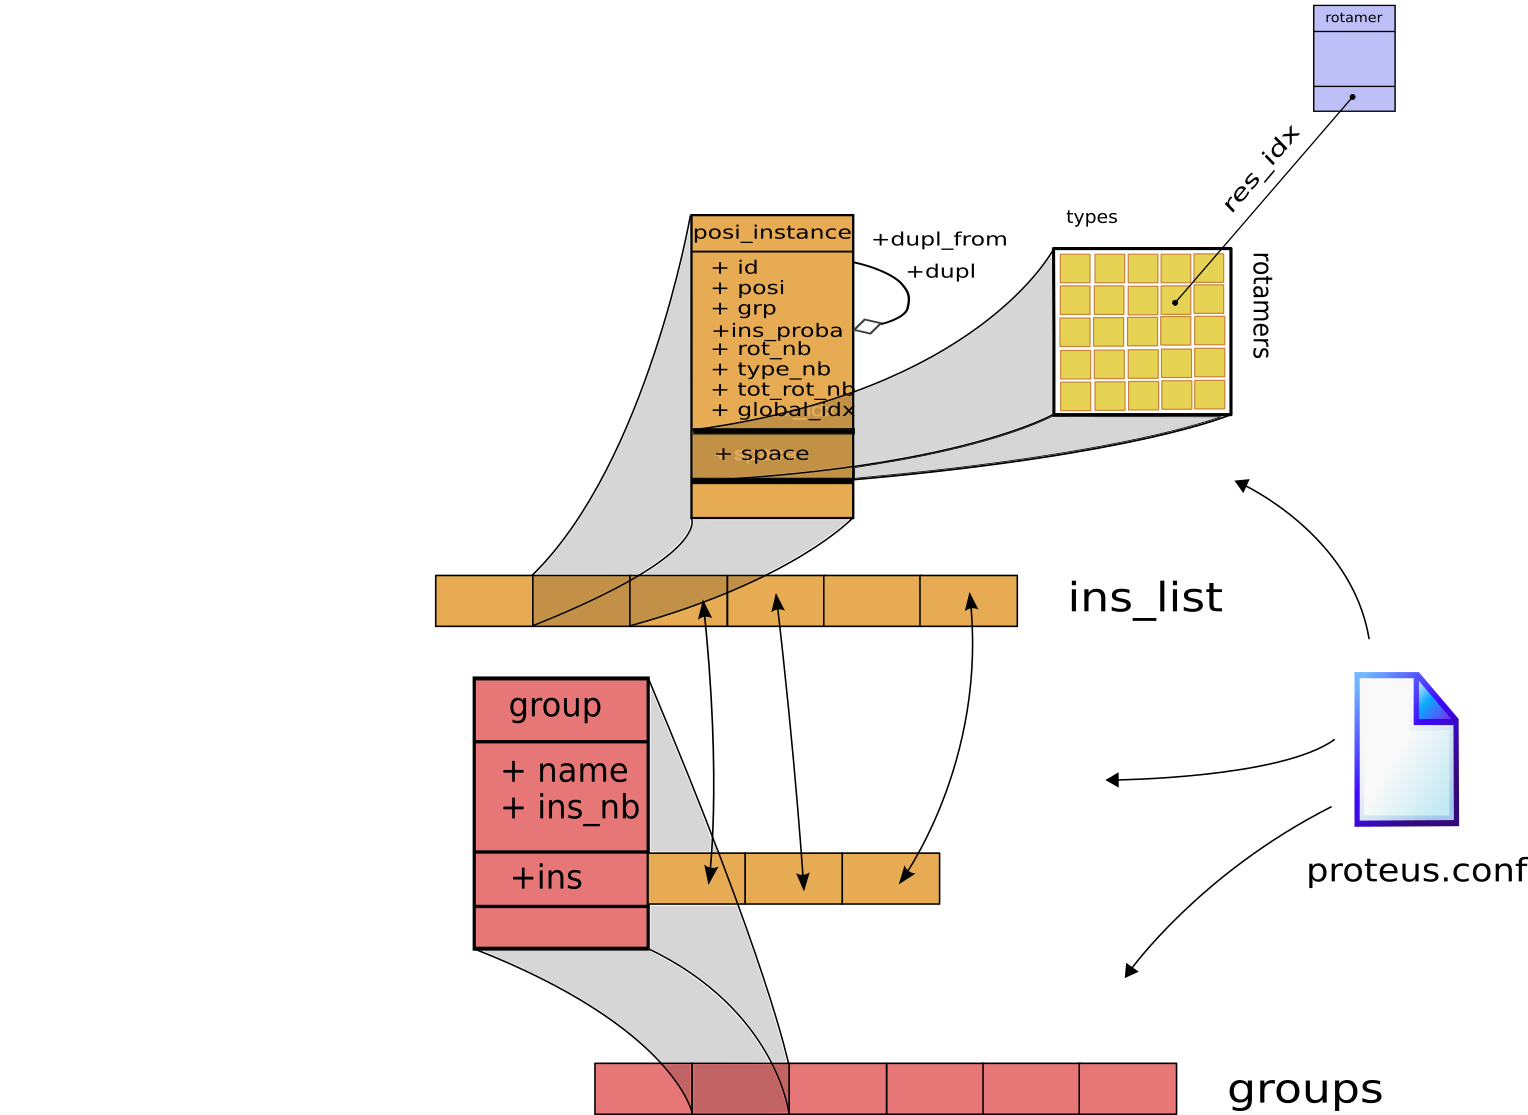
\includegraphics[width=12cm]{figure/structures_modele_logique.png} 
     \end{tabular}
     
     \caption{Les principales structures \og logiques\fg dans proteus}
\label{fig:structLog}
   \end{figure}

Le dernier ensemble de structure de données contient les éléments régulièrement modifiés au cours de l'exploration.
Il y a un tableau  \verb!grep_ener! contenant les énergies de groupes ou interactions entre groupes utilisées dans la fonction de score. La structure conformation contient la séquence-conformation courante. Une liste de structure \verb!ins_modif! qui représente les modifications à effectuer sur la conformation courante, figure \ref{fig:structDyna}.  

   \begin{figure}[!htbp]
     \centering
     \begin{tabular}{c}
       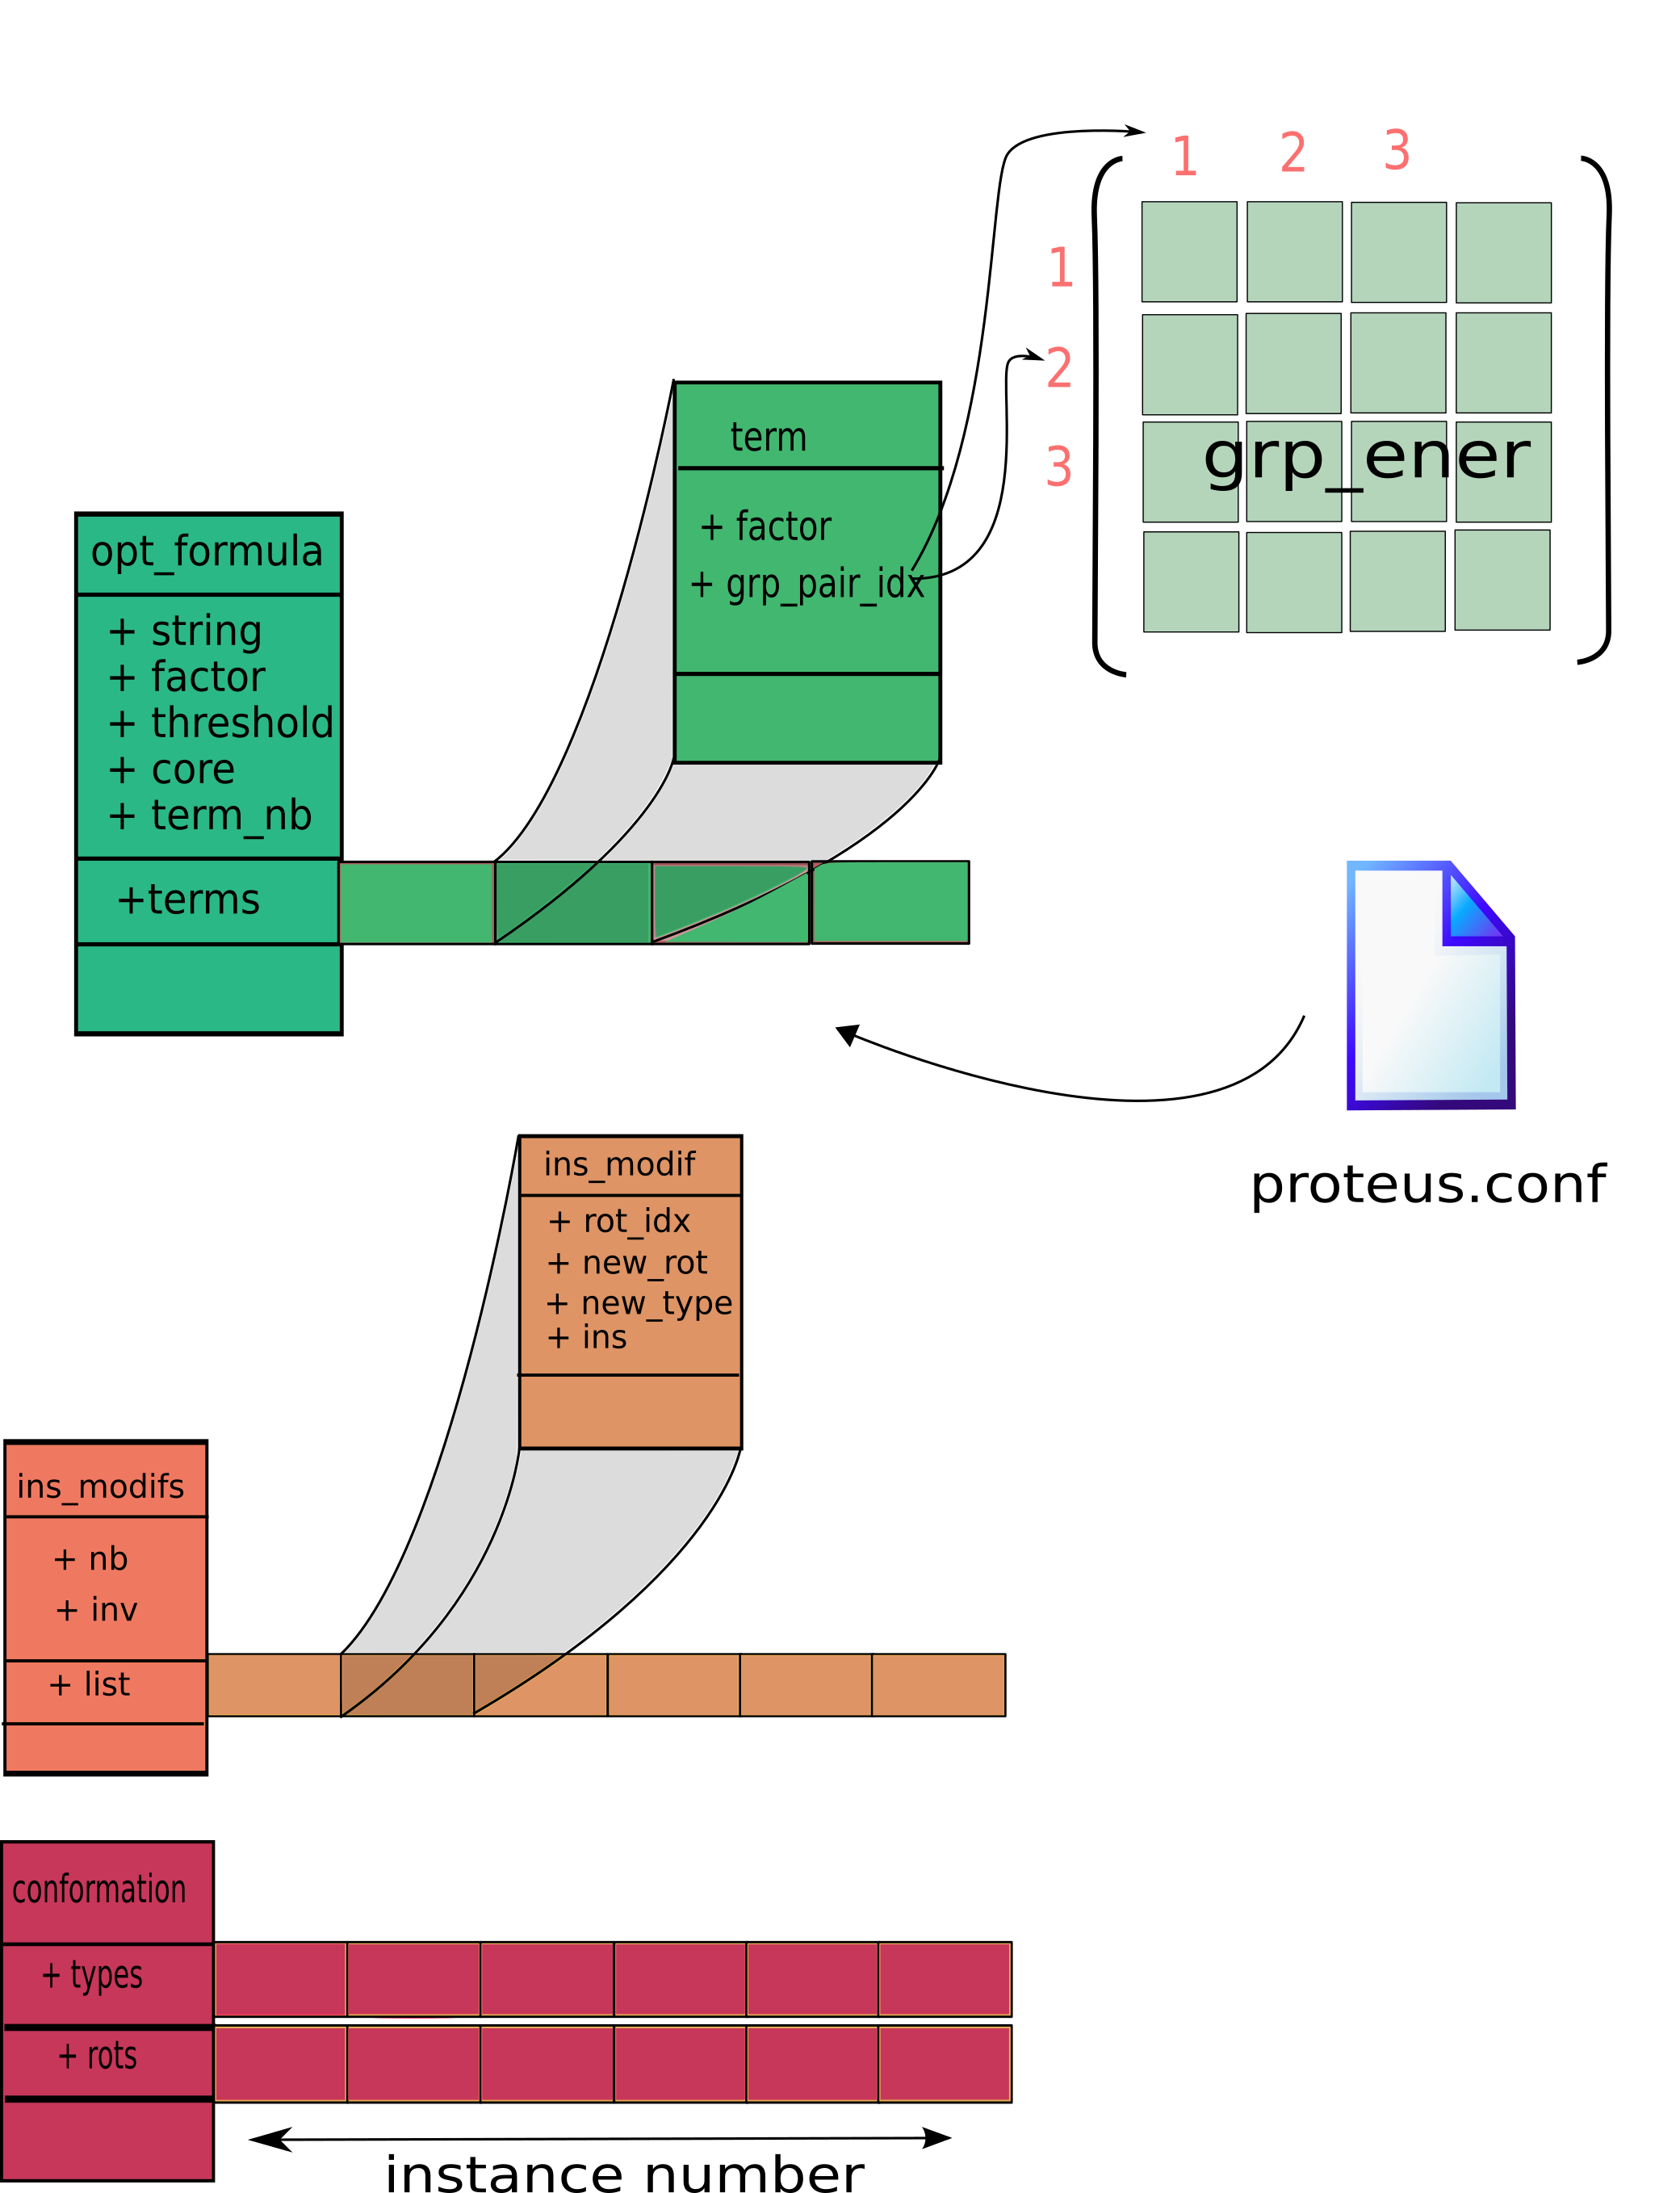
\includegraphics[width=12cm]{figure/structures_dynamiques.png} 
     \end{tabular}
     
     \caption{Les principales structures \og dynamiques\fg dans proteus}
\label{fig:structDyna}
   \end{figure}




%%% Local Variables:
%%% mode: latex
%%% TeX-master: "these"
%%% End:
